%%%%%%%% ICML 2020 EXAMPLE LATEX SUBMISSION FILE %%%%%%%%%%%%%%%%%

\documentclass{article}

% Recommended, but optional, packages for figures and better typesetting:
\usepackage{microtype}
\usepackage{graphicx}
\usepackage{subfigure}
\usepackage{booktabs} % for professional tables

\usepackage{amsmath}
\usepackage{textcomp}
\usepackage{amssymb}

% hyperref makes hyperlinks in the resulting PDF.
% If your build breaks (sometimes temporarily if a hyperlink spans a page)
% please comment out the following usepackage line and replace
% \usepackage{icml2020} with \usepackage[nohyperref]{icml2020} above.
\usepackage{hyperref}

% Attempt to make hyperref and algorithmic work together better:
\newcommand{\theHalgorithm}{\arabic{algorithm}}

% Use the following line for the initial blind version submitted for review:
\graphicspath{{assets/}}
\usepackage[accepted]{src/icml2020}

% If accepted, instead use the following line for the camera-ready submission:
%\usepackage[accepted]{icml2020}

% The \icmltitle you define below is probably too long as a header.
% Therefore, a short form for the running title is supplied here:

\icmltitlerunning{Lifelong Control of Off-grid Microgrid with Model Based Reinforcement Learning}

% Community price
\newcommand{\lowPriceCom}{\ensuremath{y^\text{com, low}}}
\newcommand{\highPriceCom}{\ensuremath{y^\text{com, high}}}
\newcommand{\impCom}[1]{\ensuremath{i^\text{com, #1}}}
\newcommand{\expCom}[1]{\ensuremath{e^\text{com, #1}}}
\newcommand{\maxImpCom}{\ensuremath{\overline{I}^\text{com}}}
\newcommand{\maxExpCom}{\ensuremath{\overline{E}^\text{com}}}
\newcommand{\expGridB}{\ensuremath{y^\text{grid, exp}}}
\newcommand{\impGridB}{\ensuremath{y^\text{grid, imp}}}
\newcommand{\expComB}{\ensuremath{y^\text{com, exp}}}
\newcommand{\impComB}{\ensuremath{y^\text{com, imp}}}

% Battery
\newcommand{\BSSs}{\ensuremath{\mathcal{B}}}
\newcommand{\OPSOC}{\ensuremath{s}}
\newcommand{\maxcharge}{\ensuremath{\overline{S}}}
\newcommand{\mincharge}{\ensuremath{\underline{S}}}
\newcommand{\chargerate}{\ensuremath{\overline{P}}}
\newcommand{\dischargerate}{\ensuremath{\underline{P}}}
\newcommand{\retentionRate}{\ensuremath{\eta^{\text{retention}}}}
\newcommand{\chargeEfficienty}{\ensuremath{\eta^{\text{charge}}}}
\newcommand{\dischargeEfficienty}{\ensuremath{\eta^{\text{discharge}}}}
\newcommand{\initialCharge}{\ensuremath{S^\text{init}}}
\newcommand{\minEndCharge}{\ensuremath{\underline{S}^\text{end}}}
\newcommand{\maxEndCharge}{\ensuremath{\overline{S}^\text{end}}}
\newcommand{\charge}{\ensuremath{P^{\text{charge}}}}
\newcommand{\discharge}{\ensuremath{P^{\text{discharge}}}}

% Devices
\newcommand{\devices}[1]{\ensuremath{\mathcal{P}^\text{#1}}}
\newcommand{\sheddableDevices}{\ensuremath{\devices{sheddable}}}
\newcommand{\flexibleDevices}{\ensuremath{\devices{flexible}}}
\newcommand{\nonflexibleDevices}{\ensuremath{\devices{non-flexible}}}
\newcommand{\steerableDevices}{\ensuremath{\devices{steer}}}
\newcommand{\nonsteerableDevices}{\ensuremath{\devices{non-steer}}}
\newcommand{\assistBatteries}{\ensuremath{\BSSs^\text{assist}}}
\newcommand{\noassistBatteries}{\ensuremath{\BSSs^\text{no assist}}}

\newcommand{\Batteries}{\ensuremath{\BSSs}}
\newcommand{\Discharge}{\ensuremath{p^{discharge}}}
\newcommand{\Charge}{\ensuremath{p^{charge}}}

% Users
\newcommand{\users}{\ensuremath{\mathcal{U}}}
\newcommand{\profit}[1]{\ensuremath{c^\text{#1}}}
\newcommand{\optprofit}[1]{\ensuremath{J^{\star, \text{#1}}}}
\newcommand{\profitshare}[2]{\ensuremath{r^{#1}(J^{\star, \text{MU}}, #2)}}
\newcommand{\netEntityPosition}{\ensuremath{p}^{\text{net}}}

% Power assist
\newcommand{\maxImport}{\ensuremath{I}^{\text{max}}}
\newcommand{\maxExport}{\ensuremath{E}^{\text{max}}}
\newcommand{\assistanceOn}{\ensuremath{y}^{\text{assist}}}
\newcommand{\assistLevel}{\ensuremath{z}^{\text{assist}}}
\newcommand{\assistedPower}{\ensuremath{p}^{\text{assisted}}}
\newcommand{\assistlevel}{\ensuremath{P}^{\text{assist}}}
\newcommand{\netPositionUB}{\ensuremath{p}^{\text{net, UB}}}


% Dual variables
\newcommand{\dualSU}[1]{\ensuremath{\lambda^\text{#1}}}
\newcommand{\dualMU}[1]{\ensuremath{\beta^\text{#1}}}

% operator
\newcommand{\operatorincome}{\ensuremath{J}^\text{operator}}

% Peak power
\newcommand{\peak}{\ensuremath{\overline{p}}}
\newcommand{\oldpeak}{\ensuremath{\overline{p}^{\text{past}}}}
\newcommand{\peakdiscount}{\ensuremath{\gamma}^{\text{peak}}}
\newcommand{\peakincrease}{\ensuremath{\delta \overline{p}}}

% Price
\newcommand{\OPprice}[1]{\ensuremath{\pi^{\text{#1}}}}

% Cost
\newcommand{\OPcost}[1]{\ensuremath{c^\text{#1}}}

% Energy
\newcommand{\exportGrid}{\ensuremath{e}^\text{grid}}
\newcommand{\OPimport}{\ensuremath{i}^\text{grid}}
\newcommand{\exportSlack}{\ensuremath{e}^\text{slack}}
\newcommand{\importSlack}{\ensuremath{i}^\text{slack}}
\newcommand{\OPexchangeOut}{\ensuremath{e}^\text{com}}
\newcommand{\OPexchangeIn}{\ensuremath{i}^\text{com}}
\newcommand{\OPprod}{\ensuremath{p^{\text{prod}}}}
\newcommand{\OPcons}{\ensuremath{p^{\text{cons}}}}

% Reserve
\newcommand{\OPreserve}[1]{\ensuremath{r^\text{#1}}}

% Time
\newcommand{\OPduration}{\ensuremath{\Delta_t}}
\newcommand{\OPperiods}{\ensuremath{\mathcal{T}}}

%Production
\newcommand{\curtail} {\ensuremath{P^\text{curt}}}
\newcommand{\steer}{\ensuremath{P^\text{steer}}}
\newcommand{\nonSteerable}{\ensuremath{P^\text{non-steer}}}
\newcommand{\steerable}{\ensuremath{P^\text{steer}}}

% Consumption
\newcommand{\shed} {\ensuremath{C^\text{shed}}}
\newcommand{\flex}{\ensuremath{C^\text{flex}}}
\newcommand{\flexCons}{\ensuremath{c^\text{flex}}}
\newcommand{\flexStart}{\ensuremath{y^\text{flex}}}
\newcommand{\flexStarted}{\ensuremath{z^\text{flex}}}
\newcommand{\exclusiveGroup}{\ensuremath{\mathcal{G}}}
\newcommand{\nonFlexible}{\ensuremath{C^\text{non-flexible}}}
\newcommand{\flexibleLoadDuration}{\ensuremath{\text{duration}^\text{flex}}}
\newcommand{\flexibleLoadProfile}{\ensuremath{\text{profile}^\text{flex}}}
\newcommand{\flexibleLoadStartTime}{\ensuremath{\text{start}^\text{flex}}}
\newcommand{\flexibleLoadEndTime}{\ensuremath{\text{end}^\text{flex}}}
\newcommand{\flexibleLoadAcceptanceRatio}{\ensuremath{\underline{a}^\text{flex}}}
\newcommand{\flexibleLoadMustRun}{\ensuremath{\text{run}^\text{flex}}}
\newcommand{\flexibleEnergy}{\ensuremath{\text{E}^\text{flex}}}
\newcommand{\sheddable}{\ensuremath{C^\text{sheddable}}}
\newcommand{\maxSheddingTime}{\ensuremath{\overline{t}^\text{shedding}}}

% Sharing
\newcommand{\weight}[1]{\ensuremath{w^\text{#1}}}

% Misc 
\newcommand{\forallt}{\ensuremath{\forall t \in \OPperiods}}
\newcommand{\forallu}{\ensuremath{\forall u \in \users}}

\begin{document}

\twocolumn[
\icmltitle{Lifelong Control of Off-grid Microgrid with Model Based Reinforcement Learning}

% It is OKAY to include author information, even for blind
% submissions: the style file will automatically remove it for you
% unless you've provided the [accepted] option to the icml2020
% package.

% List of affiliations: The first argument should be a (short)
% identifier you will use later to specify author affiliations
% Academic affiliations should list Department, University, City, Region, Country
% Industry affiliations should list Company, City, Region, Country

% You can specify symbols, otherwise they are numbered in order.
% Ideally, you should not use this facility. Affiliations will be numbered
% in order of appearance and this is the preferred way.
\icmlsetsymbol{equal}{*}

\begin{icmlauthorlist}
\icmlauthor{Simone Totaro}{equal,upf}
\icmlauthor{Ioannis Boukas}{be}
\icmlauthor{Anders Jonsson}{upf}
\icmlauthor{Bertrand Corn\'elusse}{be}
\end{icmlauthorlist}

\icmlaffiliation{upf}{Department
of Information and Communication Technologies\\ Universitat Pompeu Fabra, Barcelona, Spain.}%\\ Email: \{simone.totaro, anders.jonsson\}@upf.edu}

\icmlaffiliation{be}{Department of Electrical Engineering and Computer Science\\University of Li\`ege, Li\`ege, Belgium.} %% Email: \{ioannis.boukas, bertrand.cornelusse\}@uliege.be}

\icmlcorrespondingauthor{Anders Jonsson}{anders.jonsson@upf.edu} % ale?

% You may provide any keywords that you
% find helpful for describing your paper; these are used to populate
% the "keywords" metadata in the PDF but will not be shown in the document
\icmlkeywords{Microgrid control, optimization, reinforcement learning, dyna.}

\vskip 0.3in
]

% this must go after the closing bracket ] following \twocolumn[ ...

% This command actually creates the footnote in the first column
% listing the affiliations and the copyright notice.
% The command takes one argument, which is text to display at the start of the footnote.
% The \icmlEqualContribution command is standard text for equal contribution.
% Remove it (just {}) if you do not need this facility.

\printAffiliationsAndNotice{} % leave blank if no need to mention equal contribution
%\printAffiliationsAndNotice{\icmlEqualContribution} % otherwise use the standard text.

\begin{abstract}
	\textbf{TODO} 
	Considering data uncertainty, the problem of centralized microgrid control can be decomposed in four tasks: estimating the parameters of the microgrid devices, forecasting the consumption and the renewable production, operational planning to anticipate weather effects and human activities, and real-time control to adapt planned decision to the realization of the uncertainties. This problem becomes even more challenging in a lifelong setting. As the devices of a microgrid deteriorate over their lifetime and microgrids are by definition small systems, it is of paramount importance to automate the meta-parameterization of these stages to maximize the microgrid efficiency and decrease its maintenance costs. In this paper, we propose a novel model based reinforcement learning algorithm to address the problem of lifelong learning for off-grid microgrid control. In particular, we show that using a model allows for better exploration. The algorithm demonstrates generalisation properties, transfer capabilities and better robustness in case of changing system dynamics. The proposed algorithm is compared against a rule-based policy and a model predictive controller with look-ahead. The results show that the trained agent is able to outperform both benchmarks in the lifelong setting where the system dynamics are changing over time.
\end{abstract}

\section{ Introduction} \label{sec: Introduction}
	Microgrids are small electrical networks composed of flexible consumption, distributed power generation (renewable and/or conventional) and storage devices. The operation of a microgrid is optimized in order to satisfy the demand while ensuring maximum reliability and power quality and to maximize the renewable energy harvested locally while minimizing the total system cost.

	Centralized microgrid control is usually decomposed in four tasks: i) estimating the parameters of the microgrid devices (for instance the charge efficiency of a battery storage device as a function of the state of charge and temperature, or the actual capacity of a battery after a number of cycles), ii) forecasting the consumption and the renewable production, iii) operational planning to anticipate weather effects and human activities, and iv) real-time control to adapt planned decisions to the current situation. These tasks are preformed sequentially during the lifetime of a microgrid in order to achieve near optimal operation and to maximize the benefits arising from distributed generation. 

	The estimation of the system parameters is a critical task for the optimization of the microgrid operation. The most important parameters are the operation costs as well as the capacities of the different components and the battery efficiency \cite{Parisio2014}. This process is usually carried out using measured data and is very specific to each microgrid configuration. These parameters are then used in the simulation model where the system operation is modeled.

	After the parameters' estimation, it is important for the efficient microgrid operation to incorporate in the decision making process all the sources of uncertainty. To this end, forecasting techniques are deployed for the stochastic production and consumption. Forecasts are collected several times before the physical delivery in order to improve the accuracy of the forecasted value in the light of new information. There is a variety of forecasting techniques in the literature ranging from fundamental models of consumption and renewable energy production \cite{Dolara2015} to statistical models using measured data \cite{Lombardi2019}. 


	Subsequently, the outputs of the forecasting models in combination with the system parameters are used to compute the optimal control actions that need to be taken. The optimization of the control actions can be performed using the simulation model of the microgrid. However, the nonlinearities introduced by the system components make this problem hard to solve and without any optimality guarantees. Therefore, it is common in the literature to use a mixed integer linear approximation of the system model that can be solved easily with modern techniques and to optimality. A rolling horizon strategy is then usually adopted where the optimization is performed with some predefined look-ahead period \cite{Palma-Behnke2013}. Alternatively, a model predictive control (MPC) strategy is used for achieving economic efficiency in microgrid operation management \cite{Parisio2014}. An MPC policy is a feedback control law meant to compensate for the realization of uncertainty.

	Given the data availability, the two preceding tasks, namely forecasting and optimization, can be merged into one task and a control action can be derived directly from the data observed. To this end, reinforcement learning can be leveraged as a methodology to deal with the uncertainty and the non-linearities of the system components. The benefit from this approach is twofold: i) the nonlinearities of the simulator are accounted for in the optimization process; and ii) the training of parameters is performed in the direction of an objective function that corresponds to the system cost instead of the mean squared error as in the case of forecasting methods.

	In this paper, we present an open-source reinforcement framework for the modeling of an off-grid microgrid for rural electrification. Moreover, we formulate the control problem of an isolated microgrid as a Markov Decision Process (MDP). The degradation of the various components as well as the non-linear dynamics of several devices are considered. Due to the high-dimensional continuous action space we define a set of discrete meta-actions in a similar way to previous work~\cite{Boukas2018}.

	The main challenge for the lifelong control of an off-grid microgrid arises from the uncertainty of the future renewable production and consumption. A critical issue in microgrid operation is that oftentimes the policy learned during training on a dataset does not perform well on unseen data. Additionally, the degradation or damage of the various components such as the storage devices or the photovoltaic panels cause the previously learned policies to become suboptimal over time.

	To address these challenges we propose a novel model-based algorithm. In particular, the algorithm is an instance of Dyna \cite{sutton2012dyna}, where the model is trained using distributional losses and the policy is optimized using the Proximal Policy Optimization (PPO) algorithm. The values of the policy are updated based on the expectation computed over a set of states sampled from a model. This model is trained online using samples from the real environment. We illustrate that this algorithm allows for much better estimation of the values accounting for the uncertainties and yields enhanced exploration. Additionally, we show that the enhanced exploration gained using the model to sample states allows for better generalization to unseen data. Moreover, we show that the knowledge of a previously trained policy can be efficiently transferred when training on a new set of data. Finally, we demonstrate the ability of the controller to adapt to sudden changes such as damage of the equipment without explicit knowledge of the event. 

	To evaluate the performance of the obtained policy, we compare it with two benchmarks: i) a rule-based control that takes decisions in a myopic manner based only on current information; and ii) an optimization-based controller in which look-ahead is applied to forecast consumption and production.

	This paper is organized as follows. Section~\ref{sec: RelatedWork} elaborates on state-of-the-art methods used for microgrid operation and control. Section~\ref{sec: RLBackground} provides the theoretical background used for the developed framework and the algorithm proposed. In Section~\ref{sec: Simulator}, the system dynamics of the microgrid are detailed. In Section~\ref{sec: ProblemStatement}, we formulate the lifelong control problem of an off-grid microgrid as an MDP. Section~\ref{sec: Algorithm} presents the model-based algorithm used to solve the lifelong microgrid control problem. The proposed algorithm is compared against the two benchmark strategies presented in Section~\ref{sec: Bechmarks}. Section~\ref{sec: CaseStudy} describes the case study and results obtained. Finally, Section~\ref{sec: conclusions} concludes the main findings and provides avenues for future research.
\section{Related Work} \label{sec: RelatedWork}
	%TODO Improve

	The control of a system that includes various sources of uncertainty like the case of an off-grid microgrid heavily depends on the availability of accurate values of forecasts of the variability. Following the recent advances in artificial intelligence and the data availability, the forecasting of renewable energy sources (RES) using artificial neural networks (ANNs) has been proposed~\cite{Leva2019}, where a hybrid model combines ANNs with a Clear Sky Solar Radiation Model (CSRM) for the solar power forecasting. The resulting model is using weather forecasts and real hourly photovoltaic power data. Short-term load forecasting (STLF) for microgrids using artificial intelligence has also been proposed~\cite{Hernandez2014}, using a three-stage architecture in which a self-organizing map (SOM) is applied to the input. The outputs are clustered using the k-means algorithm, and finally demand forecasting for each cluster is performed using an ANN.

	Apart from the conventional control approaches of using a simplified model of the system and some forecasts of the variable sources to optimize the operation of the microgrid, some data-driven approaches have been proposed in the literature. One example is a modeling framework for the control of the storage device in the context of an interconnected microgrid~\cite{Kuznetsova2013}. Optimal Q-values are computed using the Q-learning method. In this setting the state and action spaces are discretized in order to reduce the computational complexity and the results show increased utilization of RES production compared to optimization methods. In the present paper, we use a more detailed representation of the system to enable more complex and expressive policies.

	Following the recent advancements in the field of Deep Reinforcement Learning (DRL), researchers have also proposed a Deep Q-learning approach for the control of seasonal storage in an isolated microgrid~\cite{franccois2016deep}. In this framework, a specific deep learning structure is presented in order to extract information from the past RES production and consumption as well as the available forecasts. Despite the highly dimensional continuous state space, the authors obtain a control policy that is able to utilize the long-term storage in a meaningful way. However, in this approach it is assumed that the dynamics of the system are linear and that forecasts of the variable resources are available.
	% maybe expand related work with modle based


\section{Reinforcement Learning Background} \label{sec: RLBackground}

\subsection{ Markov Decision Process}

    We consider an infinite horizon discounted Markov Decision Process (MDP), defined by the tuple $\langle S,A,r,\{P_t\}_t,\gamma \rangle$ where  $S$ is the state space, $A$ the action space, $r:S \times A \rightarrow \mathbb{R}$ is the Markovian cost function, $P_t: S \times A \rightarrow \Delta(S) $, $t>0$, is the transition kernel at time $t$ and $\gamma \in (0, 1) $ is the discount factor. Here, $\Delta(S)$ is the probability simplex on $S$, i.e.~the set of all probability distributions over $S$. At each time step $t$, the agent observes state $s_t \in S$, takes an action $a_t \in A$, obtains reward $r_t$ with expected value $\mathbb{E}[r_t] = r(s_t, a_t)$, and transitions to a new state $s_{t+1} \sim P_t(\cdot \rvert s_t, a_t)$. We refer to $(s_t,a_t,r_t,s_{t+1})$ as a {\em transition}. Note that we do not make any assumptions on the stationarity of the transition kernels.\\ 
    
    Let $\pi$ denote a stochastic policy $\pi : S \rightarrow \Delta(A)$ and $\eta(\pi)$ its expected discounted cumulative reward under some initial distribution $d_0\in\Delta(S)$ over states: %{\color{red} with respect to a starting state?}
    \begin{gather}
    \eta(\pi) = E_{s\sim d_0} [V_{\pi}(s)],\label{eqn: expected_cumulative_reward}
    \end{gather}
    
	\noindent
     where $\tau = \{(s_t,a_t, r_t)\}_{t \geq 0}$ is a trajectory, $p(\tau)$ is the probability distribution over trajectories,  %{\color{red} perhaps relate $p$ to $P_t$?}
     \begin{equation}
        p(\tau) = d_0(s_0) \prod_{t=0}^\infty P_t(s_{t+1} \rvert s_t, a_t) \pi(a_t \rvert s_t),
     \end{equation}{}
     
	\noindent
    and the value function $V_\pi$ is defined for each state $s\in S$ as
    \begin{gather}
        V_{\pi}(s) = E_{p(\tau)}[\sum_{t=0}^{\infty} \gamma^t r_t(s_t,a_t) \rvert s_0=s].
    \end{gather}
    The goal of the agent is to find a policy that miximizes the expected cumulative reward $\eta(\pi)$:
    %An optimal policy $\pi^{*}\in \Pi$ is a policy that maximizes the cumulative return  $\eta(\pi)$ from any starting state $s_0  \in S$: % {\color{red} again, usually defined for a state}
    \begin{gather}
    \eta^{*} = \max_{\pi} \eta(\pi),\label{eqn: optimalcost}\\
    \pi^{*} = arg \max_{\pi} \eta(\pi).\label{eqn: optimalpolicy}
    \end{gather}
    
\subsection{ Dyna}
    % this methodology
    Dyna \cite{sutton2012dyna} is a model-based reinforcement learning architecture that aims to integrate learning and planning. 
    It does so by performing online estimation of the transition kernel and reward function. For ease of exposition, let $M_\psi = \langle \hat{P}, \hat{r} \rangle$ be the parametric model learned during training. Note that we estimate a single transition kernel $\hat{P}$ even though the true kernel may not be stationary.%  {\color{red} do we really estimate one transition kernel per time step?}
    
	Algorithm~\ref{algodyna} outlines the Dyna algorithm. 
    For every transition $(s,a,r,s')$ sampled from the environment $M$, we update the parametric model $M_\psi$ via an $\textbf{update}$ function. We defer the detailed description of the update function to Section~\ref{sec: Algorithm}.
    
    After the update step, we use the learned model to perform $N$ updates of the policy $\psi$, in the same way as one would using the true environment. At every step we sample a state $s \sim d_0$, apply action $a \sim \pi( a\rvert s) $ and query the parametric model $\hat{s}', \hat{r} \sim M_\psi(s,a)$. % {\color{red} how do you sample $s$? Do you not just follow a trajectory?}
    
    Note that there are two main differences during the planning phase. First, the transition $(s, a, \hat{r}, \hat{s}')$ comes from the parametric model, and second, there is no structure in the sampling process, therefore in such an update the agent can experience any possible one step transition, even ones that are hard to gather under the current policy.
    %  update is a placeholder
    \begin{algorithm}[t]
    	\caption{Dyna}
    	\begin{algorithmic}[1]
    		\STATE \textbf{Inputs: $t=0$, $T$,$\pi_\theta$, $M$, $M_\psi$, $B$}
    		\WHILE{t $\leq$ T}
    			\STATE $s \sim M$
    			\STATE $a \sim \pi_\theta(a \rvert s)$
    			\STATE $s',r \sim M(s,a)$
				\STATE \textit{updatePolicy}$(\pi_\theta)(s,a,r, s')$
    			\STATE \textit{updateModel}$(M_\psi)(s,a,r, s')$
    			\IF{$t \geq B$}
        			\FOR{$n=0$ to $N-1$}
        				\STATE  $s \sim M(s,a)$
        				\STATE  $a \sim \pi_\theta(a \rvert s)$
        				\STATE $\hat{s}', \hat{r} \sim M\psi(s,a)$
        				\STATE \textit{updatePolicy}$(\pi_\theta)(s,a,\hat{r}, \hat{s}')$
        			\ENDFOR
        		\ENDIF
    		\ENDWHILE
    	\end{algorithmic}
    	\label{algodyna}
    \end{algorithm}
    
    
\begin{algorithm}[t]
	\caption{updatePolicy}
	\begin{algorithmic}[1]
		\STATE \textbf{Inputs}: \textit{n epochs}, $\pi_\theta$, \textit{Buffer} 
			\FOR{$n=0$ to \textit{n epochs}}
				\STATE  $s,a,r,s' \sim \textit{Buffer}$
			    \STATE  $V_{\theta_ {k+1}} = \min L(V_{\theta_k})$
			    \STATE  $\pi_{\theta_{k+1}} =  arg\max \eta (\pi_k)  + \frac{1}{\beta} D(\pi_{\theta_k} \rvert \rvert \pi_{\theta})$
			\ENDFOR
	\end{algorithmic}
	\label{update_policy}
\end{algorithm}

\begin{algorithm}[t]
	\caption{updateModel}
	\begin{algorithmic}[1]
		\STATE \textbf{Inputs}: \textit{n epochs}, $r_\psi$, $P_\psi$, \textit{Buffer} 
			\FOR{$n=0$ to \textit{n epochs}}
				\STATE  $s,a,r,s' \sim \textit{Buffer}$
			    \STATE  $P_{\psi_{k+1}} = \min L(P_{\psi_k})$
			    \STATE  $r_{\psi_{k+1}} = \min L(r_{\psi_k})$
			\ENDFOR
	\end{algorithmic}
	\label{update_model}
\end{algorithm}


\subsection{ Proximal Policy Optimization}
    
    The Proximal Policy Optimization (PPO) algorithm \cite{Schulman2017} belongs to the family of policy gradient methods and can be used with both discrete and continuous action spaces. In the vanilla actor-critic method \cite{sutton2000policy}, a parametrized stochastic policy $\pi_{\theta_k}(a_t|s_t)$ with parameters $\theta_k$, $k\geq 0$, is directly optimized towards the following regularized objective:
    
    \begin{gather}
        \eta(\pi_{\theta_k})  = \mathbb{E}_{p(\tau)}\left\lbrace 
        \frac{\pi_{\theta_k}(a_t \rvert s_t)}{\pi_{\theta_{k-1}}(a_t \rvert s_t  )} \hat{A}_{\theta_k}(s_t,a_t)\right\rbrace  - \frac{1}{\beta}  
        D( \pi_{\theta_k} \rvert \rvert \pi_{\theta_{k-1}}) ,\label{eqn: regularized}
    \end{gather}

	\noindent
	where $\hat{A}_{\theta_k}(s_t,a_t)$ is an estimator of the advantage function, $D$ is a regularizer in the form of a Bregman divergence and $\beta$ is a learning rate.
    
    After the collection of $N$ samples, a gradient step is performed for the update of the parameters $\theta$ as
    \begin{gather}
    \theta_{k+1} = \theta_{k} + \alpha \nabla \eta(\pi_{\theta_k}),\label{eqn: thetaupdatesgrad}
    \end{gather}
    
	\noindent
    where $\alpha$ is a step size. An unbiased estimator of the advantage function is given by 
    \begin{equation}
    \hat{A}_{\theta_k}(s_t,a_t) =  r(s_t,a_t) + \gamma \hat{V}_{\theta_k} (s_{t+1}) - \hat{V}_{\theta_k}(s_t), \label{eqn: advantage}
    \end{equation}
    
	\noindent
    where the value function $\hat{V}_{\theta_k}$ is obtained by minimizing the following loss:
    % not sure if this an estimator
    \begin{equation}
        L(\hat{V}_{\theta_k}) = \frac{1}{2} \mathbb{E}_{p(\tau)} [ \hat{A}_{\theta_k}(s_t, a_t)^2]
    \end{equation}{}

    In practice we always optimize multiple epochs of mini-batch updates of stochastic gradient descent of both objectives.
\subsection{Quantile Regression}

	% \noindent
	% {\color{red} Explain how this relates to the previous theory. Where do the distributional losses fit in the theory? The only loss you have described earlier is the one in Equation (6). Also do not use citations as nouns! (e.g. [14] introduced; it is written in [15], etc.)}

	Model based reinforcement learning requires an estimator of the transition function $P_t$ and the reward function $r_t$. It is a common practice to treat this problem as supervised learning use the square loss to build an estimator for each of those function separetely.

	Distributional losses introduced in \cite{bellemare2017distributional} and expanded \cite{dabney2018distributional} achieved state of the art performance in several reinforcement learning benchmarks. \cite{imani2018improving} discusses the importance of distributional losses for regression problem arguing that such losses have locally stable gradients which improves generalization. Here we concisely report the loss function for our setting. For a more detailed description the reader can consult \cite{dabney2018distributional}. 
	Our goal is to learn the distribution of some random variable $z \sim F(z)$. To do so, its known that the value of the quantile function $F^{-1}_z(\tau)$ is the minimizer of the quantile regression loss. Let $(-k, k)$ be the support of the empirical CDF then the Quantile Huber loss is defined as:

		\begin{equation}
			\rho_{\tau}(u) = \lvert \tau - \delta_{\{u\leq0\}}\rvert L(u)
		\end{equation}
	Where $L(u)$ is given by:
		\begin{equation}
			L(u) = 
			\begin{cases}
				\frac{1}{2} u^2,& \text{if} \lvert u \rvert \leq k \\
				k(\lvert u\rvert - \frac{1}{2}k),& \text{otherwise}
			\end{cases}
		\end{equation}

\section{Microgrid Description}\label{sec: Simulator}
    \label{sec:gym}
    % find another notation !!!
    In this section we provide a detailed description of the system considered. An off-grid microgrid designed for rural electrification is inherently characterized by changes occuring in different time-scales. We provide a formal description of the differnt types of changes and we motivate the need for a lifelong control that has the abitility to adapt to these changes.
    
    
\subsection{Components}

An off-grid microgrid is composed of the following components:
 
\subsubsection{Consumption} 
    
    The consumption of the isolated microgrid $\nonFlexible$ is considered to be non-flexible, meaning that there is a high cost associated to the energy non-served. The consumption $\nonFlexible_{t}$ at each time-step $t$ of the simulation is assumed to be a stochastic variable sampled from distribution $P^{C}_{t}$ given the $h$ previous realizations according to:
    \begin{gather}
    \nonFlexible_{t} \sim P^{C}_{t}( \nonFlexible_{t-1}, ...,\nonFlexible_{t-h} ).\label{eqn: load}
    \end{gather}
    In this paper, it is represented by real data gathered from an off-grid microgrid. The distribution $P^{C}_{t}$ is indexed in time in order to indicate that changes occur in the aggregate consumption over the life-time of the microgrid. For instance, a change in the consumption profile can be caused by the fact that more users are progressively connected to the micro-grid.

\subsubsection{Storage model}
    
    The modeling of the storage system can become quite complex and highly-nonlinear depending on the degree of accuracy required by each specific application. In this paper, we use a linear ``tank'' model for the simulation of the battery since we assume that the simulation time-step size $\Delta t$ is large enough (1 hour). The dynamics of a battery are given by
    \begin{gather}
    SoC_{t+1} = SoC_{t}+ \Delta t\cdot(\chargeEfficienty \charge_t - \frac{\discharge_t}{\dischargeEfficienty}) ,\label{eqn: storagedynamics}
    \end{gather}
    where $SoC_{t}$ denotes the state of charge at each time step $t$, $\charge$ and $\discharge$ correspond to the charging and discharging power, respectively and $\chargeEfficienty$, $\dischargeEfficienty$ represent the charging and discharging efficiencies of the storage system. The charging ($\charge$) and discharging ($\discharge$) power of the battery are assumed to be limited by a maximum charging rate $\chargerate$ and discharging rate $\dischargerate$, respectively. Accounting for the storage system degradation, we consider that the maximum capacity $\maxcharge$ of the storage system as well as the charging and discharging efficiencies ($\chargeEfficienty$, $\dischargeEfficienty$) are decreasing as a linear function of the number of cycles $n_t$ that are performed at each time-step $t$. We have, $\forall t \in T$, 
    \begin{align}
    SoC_{t}, \charge_t, \discharge_t &\geq 0 \\
    \charge_t &\leq \chargerate\\
    \discharge_t &\leq \dischargerate , \\
    SoC_{t} &\leq \maxcharge \label{eqn: storage limits},\\
    \maxcharge&=s(n_t). \label{eqn: storage_limits_evolving}
    \end{align}
    

\subsubsection{Steerable generator model}
    Steerable generation is considered any type of conventional fossil-fuel based generation that can be dispatched at any time-step $t$. When a generator is activated, it is assumed to operate at the output level $\steer_t$ that is ranging between the minimum stable generation $\underline{\steerable}$ and the maximum capacity $\overline{\steerable}$ such that
    \begin{gather}
    \underline{\steerable} \leq \steer_t \leq \overline{\steerable}.\label{eqn: generatordynamics}
    \end{gather}
    The fuel consumption $F_t$ related to the operation of the generator at time $t$ is a linear function of the power output $\steer_t$ curve with parameters $F_1$, $F_2$ given by the manufacturer. 
    \begin{gather}
    F_t = F_1 + F_2 \cdot \steer_t .\label{eqn: fuelconsuption}
    \end{gather}
    The fuel cost $\profit{fuel}_t$ accounting for the fuel price $\OPprice{steer}$ is then given by:
    \begin{gather}
    \profit{fuel}_t = F_t \cdot \OPprice{fuel} .\label{eqn: generatorcost}
    \end{gather}
    
\subsubsection{Non-steerable generators model}
    The level of non-steerable generation from renewable resources such as wind or solar is denoted by $\nonSteerable$. Similar to the non-flexible load case it is assumed that $\nonSteerable_t$ at time-step $t$ is sampled from a probability distribution $P^{\nonSteerable}_{t}$ given the $h$ previous realizations according to:
    \begin{gather}
    \nonSteerable_t \sim P^{\nonSteerable}_{t}( \nonSteerable_{t-1},...,\nonSteerable_{t-h}).\label{eqn: pv}
    \end{gather}
    In this paper, this is represented by real data gathered from an off-grid microgrid. Similar to the case of the non-flexibel load the distribution $P^{\nonSteerable}_{t}$ is indexed by time $t$ to indicate that changes in the renewable production might occur over time. These changes are mostly related to the progressive degradation of the equipment (solar panels).
    
\subsubsection{Power balance}
    At each time-step $t$ in the simulation horizon we can compute the power balance between the injections and the off-takes. The residual power $P_t^{RES}$ resulting from the mismatch between production and consumption is curtailed $\curtail_t$ if its positive and shed $\shed_t$ if it is negative. We can formally define the power balance as:
    \begin{gather}
    \nonSteerable_t + \steer_t + \discharge_t - \charge_t - \nonFlexible_t\\\notag
    =\curtail_t - \shed_t,\label{eqn: powerbalance}
    \end{gather}
    with $\curtail_t , \shed_t \geq 0$.
    The costs arising from the curtailment of generation or the shedding of non-flexible loads are given by: 
    \begin{gather}
    \profit{curt}_t = \curtail_t \cdot \OPprice{curt} \label{eqn: curtcost}
    \end{gather}
    \begin{gather}
    \profit{shed}_t = \shed_t \cdot \OPprice{shed} \label{eqn: shedcost}
    \end{gather}
    


\subsection{Characterizing changes in the environment}
	
	Oftentimes in real-life applications the concept of interest depends on some underlying context that is not fully observable. Changes in this underlying concept might induce more or less radical changes in the concept of interest, which is formally known as concept drift \cite{tsymbal2004problem}. For instance, in the off-grid microgrid under study the connection of new users and their habits have strong influence on distribution $ P^{C}_{t}$. However, it is not possible to know exactly and to quantify the effect on the consumption a priori. 
	
	The extent of the drift is defined as the rate of change of the underlying distribution in two subsequent time instances and it is used to characterize the concept drift. Let $P_{t}$ be the underlying probability distribution. Computing the extent of the drift essentially boils down to computing the difference between two distributions using a distance measure (e.g. KL divergence) $D(P_{t+1}||P_{t})$.
	In this paper, we deal with the following two distinct set of changes:
	
	\subsubsection{Gradual changes}
	These are cases in which a slow concept drift occurs. The extent of the drift is bounded so that any learner can follow these changes successfully. A formal bound on the maximal rate of drift that is acceptable by a memory-based learner is given in \cite{kuh1991learning}.
	
	In this paper we assume that changes related to the consumption and renewable production profiles as well as degradation of the equipment (storage) belong to this category.
	
	\subsubsection{Sudden or abrupt changes}
	These are cases in which the extent of the drift exceeds the maximal rate and consequently a learner cannot adapt to the change. In the concept of an off-grid micro-grid this type of change would typically occur during equipment failure. 

\section{Problem Statement} \label{sec: ProblemStatement}

    The operation of the system described in section \ref{sec: Simulator} can be modelled as a Markov Decision process as it is defined in section \ref{sec: RLBackground}. We consider that at each time-step $t \in T$ the state variable $s_t \in S$ is composed of a deterministic and a stochastic part as $s_t = \left(s_t^{d}, s_t^{s}\right) \in S$ and contains all the relevant information for the optimization of the system. The deterministic part $s_t^{d} = \left(SoC_{b,t},\forall b \in \mathcal{B}\right) \in S^{d}$ corresponds to the evolution of the state of charge of the storage devices and can be fully determined by Equations (\ref{eqn: storagedynamics})-(\ref{eqn: storage_limits_evolving}). The stochastic variable $s_t^{s}$ represents the variable renewable production and consumption as $s_t^{s} = \left(\left(\nonFlexible_t,...,\nonFlexible_{t-h}\right), \left(\nonSteerable_t,...,\nonSteerable_{t-h} \right)\right) \in S^{s}$ as defined in Equations (\ref{eqn: load}) and (\ref{eqn: pv}).
    
    The available control action $a_t$ that can be applied at each time-step $t$ is defined as:
    \begin{gather}
    a_t= \left((\discharge_{b,t},\charge_{b,t}, \forall b \in \mathcal{B}), (\steer_{g,t}, \forall g \in \mathcal{G}) \right) \in A,
    \end{gather}
    and contains the charging/discharging decisions for the storage systems and the generation level of the steerable generators.
    
    At each time-step $t$ the system performs a transition based on the dynamics described in Section~\ref{sec: Simulator} according to
    \begin{gather}
    s_{t+1}^{d} = f_{t}\left(s_t, a_t\right), \label{eqn: transitionfunction}\\
    s_{t+1}^{s} \sim P^{s}_{t}\left(s_t^{s}\right)\label{eqn: stochastic_probabilities},
    \end{gather}
    where $f_{t}$ is a deterministic function and $P^{s}_{t}$ is used to denote the joint probability distribution of the stochastic variables $\nonFlexible, \nonSteerable$ as defined in Equations (\ref{eqn: load}) and (\ref{eqn: pv}). Note that the transition function $f_{t}$ is indexed in time to account for the changes (e.g. degradation) of the equipment. Equations (\ref{eqn: transitionfunction}) and (\ref{eqn: stochastic_probabilities}) can fully determine the transition kernel of the MDP at each time step as $P_t: S \times A \rightarrow \Delta(S)$.
    
    Each transition generates a negative reward (cost) $r_t$ according to the reward function $\rho(s_t, a_t) \in \mathbb{R}$, defined as:
    \begin{gather}
    r_t = \rho(s_t, a_t) = -(c_f + c_{curt} + c_{sh}).\label{eqn: rewardfunction}
    \end{gather}
    

    The problem of life-long control of an off-grid microgrid is equivalent to finding a policy $\pi$ that miximizes the expected cumulative reward $\eta(\pi)$ defined in equations (\ref{eqn: expected_cumulative_reward})-(\ref{eqn: optimalpolicy}).

    \subsection{Microgrid Simulator}
    The described MDP for off-grid microgrid control is available as an open source simulator\footnote{Available at \url{https://github.com/bcornelusse/microgridRLsimulator}.}implemented in OpenAI gym \cite{brockman2016openai}. The simulator contains a detailed modelling of the microgrid components and allows for applying any control strategy. It receives as input the microgrid configuration (components size and parameters, time series representing the exogenous information, and simulation parameters) and simulates the operation for a predefined simulation horizon $T$.

\section{Algorithm} \label{sec: Algorithm}
        % - genearlize
        % - learn
        
        Real world applications are non-stationary, partially observable and high dimensional. A desirable algorithm should effectively deal with those challenges as well as provide basic safety guarantees \cite{dulac2019challenges}.
        
        Model Based RL algorithms are appealing for real world application because they are sample efficient, they explicitly approximate the environment dynamics, and, when combined with powerful function approximation, they can scale to the high dimensional setting \cite{nagabandi2018neural}.
        
        The key issue with Model Based RL is learning the model sufficiently well to be useful for policy iteration. For real world application, this issue is worsened by the requirements of generalisation and sample efficiency.
        
        To address those challenges we propose a practical algorithm that builds upon the Dyna architecture \cite{sutton2012dyna}.
        We use a variant of PPO \cite{Schulman2017} to perform policy iteration, and quantile losses to approximate the model dynamics. We have two quantile losses, one for learning the transition kernel $P_\psi$ and one for the learning the reward function $r_\psi$:

		%{\color{red} explain these equations!}
        
        \begin{align}
        	L^P(s) &= E[\sum_{i=1}^q \rho_{\tau_i}(s' - P_\psi(s,a)], \\
        	L^r(r) &= E[\sum_{i=1}^q \rho_{\tau_i}(r - r_\psi(s,a)].
        \end{align}
        
        Model free updates are performed in PPO by sampling a partial trajectory and directly maximing {\eqref{update_policy}}. %{\color{red} (sentence seems incomplete?)}
        We use two seperate networks for the value and the policy, and we select the advantage estimator as in~\eqref{eqn: advantage}. Model based updates are one-step simulated transitions. As noted in previous work~\cite{van2019use}, updating simulated states helps to empirically mitigate model error, constraining it to simulated states. Complementary work~\cite{janner2019trust} shows that simulating one-step transitions provides a strong baseline with respect to partial or complete policy rollouts with a learned model, and PPO mantains its monotonic improvement property.
        
        In practice, in order to deal with the high dimensionality of the state and action space, we represent the model $M_{\psi}$ as a neural network with shared parameters $\psi \in \Psi$ and two heads $P_\psi$ and $r_\psi$. Each head outputs a vector of size $d \times q$ where $d$ is the output dimension and $q$ is the number of quantiles considered.
        %{\color{red} (should be $M_\psi$ no?)} 
        The policy $\pi_\theta(a\rvert s)$ and the value function $V_\theta'(s)$ are represented using two different networks. Contrary to previous claims~\cite{Schulman2017}, sharing parameters does not seem to improve learning.
        Finally we introduce hyper parameters $B \in \mathbb{N}$ that is the minimum amount of optimisation performed with the model prior to allowing model-based updates. Empirically we found this to reduce the detrimental effect of model error on policy updates. We refer to the presented algorithm as $D-Dyna$.
        
   \section{Benchmark strategies} \label{sec: Bechmarks}

In this section we introduce two control strategies used for comparison purposes. First a myopic rule-based strategy is used to provide an upper bound of the total operational cost in the period considered. The second strategy corresponds to a model-predictive control (MPC) with $N$-step look-ahead where full knowledge about the future is assumed. If the number of look-ahead steps is sufficiently large we can obtain a lower bound on the total costs.

\subsection{Rule-based controller}
The rule-based controller is a simple myopic controller that implements a set of decision rules to determine the control actions that need to be taken at each time-step $t$. It requires only data regarding the present condition of the microgrid. The logic that is implemented is the following:
\begin{enumerate}
	\item First, the difference between the current total RES production and non-flexible demand is computed: $$P_t^{RES} = \nonSteerable_t - \nonFlexible_{t}$$
	\item If $P_t^{RES}$ is positive, the status of every battery $b \in \mathcal{B}$ is set to charge ($``C"$) and the vector $y_t$ is formed as:
		$$y_t = (``C", \forall b \in \mathcal{B})$$
	\item If $P_t^{RES}$ is negative, the status of every battery $b \in \mathcal{B}$ is set to discharge ($``D"$) and the vector $y_t$ is formed as:
	$$y_t = (``D", \forall b \in \mathcal{B})$$
	\item When the vector $y_t$ is fixed, the residual generation is dispatched over devices as presented in Algorithm \ref{algoRBC}, and the decision variables related to the storage devices ($\discharge_{b,t},\charge_{b,t}, \forall b \in \mathcal{B}$) and the generators ($\steer_{g,t}, \forall g \in \mathcal{G}$) are determined. 
\end{enumerate}

\begin{algorithm}[t]
	\caption{Power dispatch.}
	\begin{algorithmic}[1]
		\STATE \textbf{Inputs: $P_t^{RES}$ , $y_t = (b.Status, \forall b \in \mathcal{B})$}
		\IF{ $P_t^{RES} \geq 0 $}
		\FORALL{$b \in \mathcal{B}$} 
		\IF{ $b.Status = "C" $}
		\STATE $\charge_t = \min(P^{RES},\chargerate)$ 
		\ENDIF
		\STATE $P_t^{RES} \leftarrow P_t^{RES} - \charge_t$
		\ENDFOR
		\ELSE
		\FORALL{$b \in \mathcal{B}$} 
		\IF{ $b.Status = "D" $}
		\STATE $\discharge_t = \min(-P^{RES},\dischargerate)$ 
		\ENDIF
		\STATE $P_t^{RES} \leftarrow P_t^{RES} +\discharge_t$
		\IF{ $P_t^{RES} \leq 0 $}
		\STATE $\steer_t=P_t^{RES}$
		\ENDIF
		\ENDFOR
		\ENDIF
	\end{algorithmic}
	\label{algoRBC}
\end{algorithm}

\subsection{Optimization-based controller}\label{sec: optcontroller}
    The optimization-based controller receives as input all the parameters available such as the future renewable production and the electrical demand, state of charge of the storage systems, components parameters, etc., and solves an optimization problem with $N$-step look-ahead. At each control time-step $t$ the objective function aims at minimizing the curtailment, load shedding and fuel costs (the $\pi$ parameters denote unit costs):
    \begin{align}
    \min &\ \OPduration \sum_{k=0}^{N} \bigg(\sum_{g\in \nonsteerableDevices} \OPprice{curt}_g \curtail_{g, t+k} + \sum_{d \in \nonflexibleDevices} \OPprice{shed}_d \shed_{d, t+k} \notag \\
    & \quad \quad \quad \quad + \sum_{g \in \mathcal{G}}   \OPprice{fuel}_g \left(F_{g, 1} + F_{g, 2} \steer_{g, t+k}\right) \bigg).
    \end{align}
    The energy balance constraints for each look-ahead step $k=0,...,N$ can be written as:
    \begin{align}
    & \sum_{g \in \mathcal{G}} \steer_{g,t+k}
    + \sum_{g\in \nonsteerableDevices} (\nonSteerable_{g,t+k} - \curtail_{g,t+k}) \notag + \sum_{b\in\Batteries} \discharge_{b,t+k} \\
    & = \sum_{b\in\Batteries} \charge_{b,t+k} + \sum_{d \in \nonflexibleDevices}  (\nonFlexible_{d,t+k} -\shed_{d,t+k}) \label{eq:net_position} 
    \end{align}
    The non-negative variables $\charge_{b,t+k}$ and $\discharge_{b,t+k}$ are bounded above by the maximum charging $\chargerate_b$ and discharging $\dischargerate_b$ power of battery $b$, respectively. 
    For each generator $g$, the fraction of the non-steerable power generation $\nonSteerable_{g,t+k}$ that is curtailed and the fraction of steerable generation $\steerable_{g,t+k}$ that is activated are represented by $\curtail_{g,t+k}$ and $\steer_{g,t+k}$, respectively. Binary variables $k_{g,t+k}$ are added to the model for the minimum operating point of the steerable generators:
    \begin{equation}
    k_{g,t+k} \underline{\steerable_{g}} \leq \steer_{g,t+k} \leq  k_{g,t+k} \steerable_{g}
    \end{equation}
    The transition law of the state of charge $s$ of each battery $b$ is modelled as in (\ref{eqn: generatorcost}).
    Overall, the problem is a mixed-integer linear program.

\section{Case study}\label{sec: CaseStudy}

\subsection{System configuration}

The evaluation of the developed methodology is performed using empirical data measured by the off-grid micro-grid system of the village ``El Espino" (-19.188, -63.560), in Bolivia, installed in September 2015 and composed of 60kW of photovoltaic (PV) panels, 464kWh of battery storage and a 58 kW generator. The system serves a community of 128 households, a hospital and a school, as well as the public lighting service. A comprehensive description of the system and of the data is available in previous work~\cite{Balderrama2019}. Aggregate electric load data is available as an indirect measure, i.e. as the sum of direct measurements retrieved from PV arrays, Gen-Set and batteries by means of smart meters. 
The parameters used for this specific microgrid configuration are given in Table \ref{input_param}. It is important to note that the minimum stable generation level is rather high due to local regulations: the very low diesel price is due to a state subsidy, but the state restricts the operation of all the conventional generators below 80\% of their nominal capacity in order to operate close to the optimal efficiency. This restriction imposes a large discontinuity in the microgrid operation and is further discussed in the results section.

\begin{table}
	\begin{center}
		\renewcommand\arraystretch{1}
		\caption{Input parameters.}
		\begin{tabular}[b]{l r r}
			\hline
			$\maxcharge$ & 120 & kWh \\
			$\chargerate$, $\dischargerate$ & 60 & kW \\
			\chargeEfficienty, \dischargeEfficienty & 95 \% \\ 
			$\OPprice{fuel}$ & 1 & \texteuro/kWh\\
			$\OPprice{curt}$ & 1.5 & \texteuro/kWh \\
			$\OPprice{lost load}$ & 10 & \texteuro/kWh \\
			$\OPduration$ & 1 & h\\
			$\overline{\nonSteerable}$ & 60 & kW \\
			$\overline{\steerable}$ & 58 & kW \\
			$\underline{\steerable}$ & 46.4 & kW \\
			\hline
		\end{tabular}
		\label{input_param}
	\end{center}
\end{table}

	\subsection{\textbf{TODO} Partial Observability}
	    The stochastic component of the transition kernel is known to be not markovian and the optimal decision requires the knowledge of the next $t+l$ times.
	    In supervised learning, state based networks as are the de facto standard \cite{taylor2018forecasting}.
		We take a similar approach as the one take for the optimization based controller \ref{sec: optcontroller} and use the model as a 1-step forecaster. After the warmup iterations $B$ we augment the current state with the prediction of the next $t+l$ given by the model.

	\subsection{\textbf{TODO} Action Space and Meta-Actions}
		% it is important to observe that this helps the RL agent but it imposes a sever restriction over the space of possible policies. 
		% we need this to explain the difference in performance between our agent and the mpc
	Due to the continuous and high dimensional nature of the state and the action spaces of the problem, reinforcement learning methods cannot be applied in their exact form. However, recent developments in the field of reinforcement learning have made possible the design of approximate optimal policies using function approximation.

	In our setting function approximation alone is not enough. The action space exploited by an optimal controller \ref{sec: optcontroller} in figure \ref{fig:action-space} is constrained to a subset of the polytope.
	
	Therefore  we elaborate on the design of a small and discrete set of actions $A'$ that maps to the original action space $A$.  This step is necessary for the use of policy-based algorithms, as the minimization problem defined in \eqref{eqn: optimalpolicy} is hard to solve. Each of the storage devices can have status $y_{b,t}\in Y$ of charging, discharging or idling where $Y= \left\lbrace ``C",``D", ``I" \right\rbrace $. We define a discrete action $a'_{t} \in A'$ that can take values from all the possible combinations of $y_{b,t}$ as:
		\begin{gather}
		a'_{t} = (y_{b,t}, \forall b \in \mathbb{B}) \in Y^{|B|}
		\end{gather}
		
		Defining the action space in this way allows the use of the dispatch rule defined in algorithm \ref{algoRBC} to obtain the control actions $a_t$.

	The describe action space $A'$ simplify the problem but it restricts the class of possible policies substantially harming the performance of the reinforcement learning methods. We leave treating the action space as a future work.

\begin{figure}[t]
	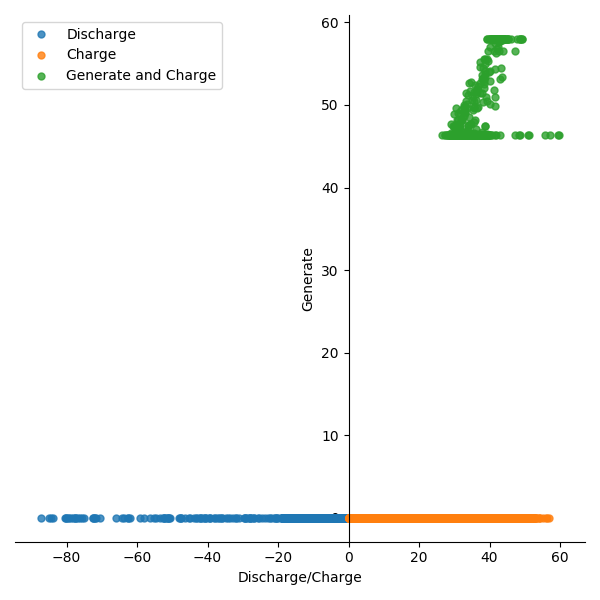
\includegraphics[width=0.4\textwidth]{action_space.png}
	\centering
	\caption{Action space covered by the optimization-based controller \ref{sec: optcontroller}.}
	\label{fig:action-space}
\end{figure}

\subsection{Comparison with the benchmarks}
% rule basd
% mpc + 1h (~ model based)
% model free
% model based

The algorithm is compared against the two benchmarks described in Section \ref{sec: Simulator} and the simple model free version of PPO \cite{Schulman2017}. We denote $PPO$ the baseline algorithm which only performs model free updates and $D-Dyna$ our method.
Three variants of the optimization controller were considered for comparison purposes. First, an optimization controller with perfect knowledge and 12 periods of look-ahead is considered in order to obtain a good approximation for the lower bound of the control problem. Second, an optimization controller with 12 periods of look-ahead and additional noise around the exact value of the stochastic variables. Third, a myopic optimization controller with no period of look-ahead was considered.

Training step on the x-axis is the number of times a new set of trajectories has been used for computing one or multiple gradient step. For a fair comparison we fix the total number of samples available for the agent and compute the number of samples per training update accounting for the number of gradient step and the number of planning steps. Finally repoults are averated of 10 seeds where stochasticity is taken into account.

\subsection{\textbf{TODO} Generalization}
% explain what is generalization
% how you test generalization and why
% show and discuss results


One of the challenges of real world applications is the occurrence of a change in the transition dynamics. As described in Section \ref{sec: Simulator}, the dynamics of the microgrid are composed of a deterministic part and a stochastic part. The stochastic part is not controllable and therefore constitutes a source of progressive change. 
An algorithm that generalizes over an unseen data distribution can provide a good initialization for fine-tuing of the new controller.
The following protocol was carried out for the training and the evaluation of the proposed algorithms. We split dataset in training set and test set: the training set lasts from January 2016 to December 2016, while the test set lasts from January 2017 to July 2017. 

As illustrated in Figure~\ref{fig:rl-results}, introducing a model benefits generalization and both the baseline and our algorithm are comparable with the heuristic. We conjecture that updating imagined states does not harm learning and gives a wider coverage of the state, action space manifold, making the algorithm generalize.

\begin{figure}[t]
	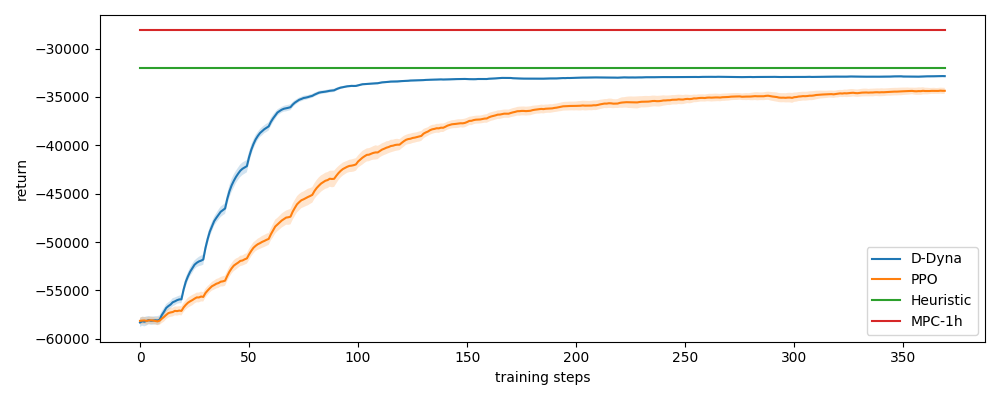
\includegraphics[width=0.5\textwidth]{generalization.png}
	\centering
	\caption{Cumulative return on the test set.}
	\label{fig:rl-results}
\end{figure}

\subsection{\textbf{TODO} Robustness}

As a next step, we consider a change in the deterministic component of the transition dynamic.
The change depicted here it is sudden and may compromise the overall functioning of the dynamic. An example of such change is the exclusion of the battery from the grid system. Let $X \sim Exp(\lambda)$ be the random variable modelling such a change. If the battery is disconnected then $soc=0$, since the controller can not store energy and must find the best allocation. For simplicity, the battery is brought back after a fixed period of T hours.

Under this scenario we evaluate the rule-based system, the model-free method as well as the model based method.

As we can see in Figure~\ref{fig:change}, the rule-based system performs very poorly while our algorithm is able to quickly adapt to the new drastically changed dynamics.

    
    \begin{figure}[t]
    	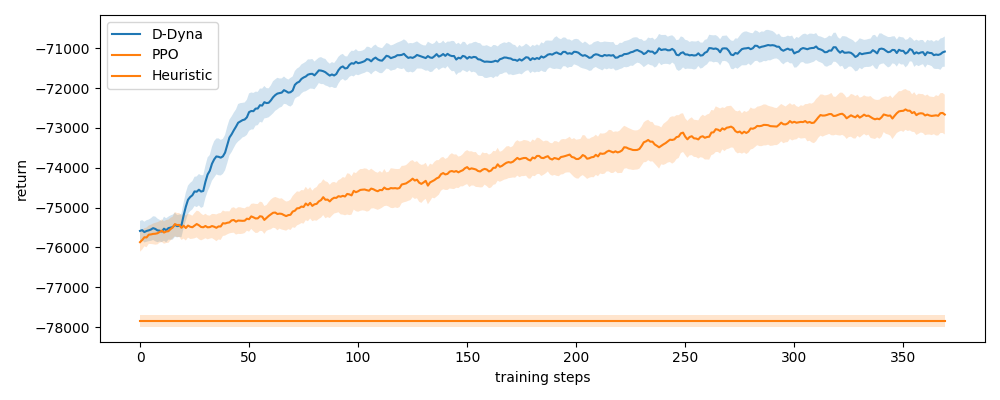
\includegraphics[width=0.5\textwidth]{robustness.png}
    	\centering
    	\caption{Cumulative return when the battery is excluded.}
		\label{fig:change}
    \end{figure}
    

\subsection{\textbf{TODO} Transfer}

    In Reinforcement Learning, transfer learning is the ability of speeding up learning on new MDPs by reusing past experiences between similar MDPs. For real world scenarios, we would like to have an algorithm that can learn off-line and adapt as the task changes. 


    A natural instance of such feature is to consider each month as a separate MDP and evaluate the ability to transfer knowledge across months. Note that each month has a different distribution of the stochastic component of the transition kernel.
    
	We set up the following experimental protocol. We use January 2016 to pre-train the algorithms, while February and August 2016 are chosen as the evaluation tasks. Intuitively transfer should be easier if the data distributions are close in time, and harder otherwise.
	
    The results of the described protocol are presented in Figures~\ref{fig:transfer-feb} and~\ref{fig:transfer-aug}. As we can see, transferring the model and the control allow better performance than learning from scratch. We identify as $-Transfer$ weather the algorithm has been pretrained. Also in this case, the model based method speeds up learning substantially.


    \begin{figure}
     	\centering
     	\begin{minipage}{0.6\textwidth}
     		\centering
     		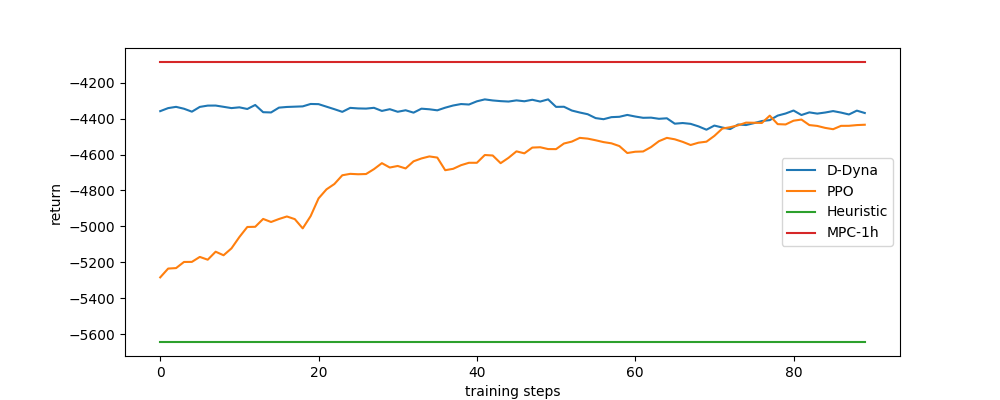
\includegraphics[width=0.8\textwidth]{feb.png}
     		\caption{Cumulative return on February.}
			\label{fig:transfer-feb}
     	\end{minipage} \hfill
     	\begin{minipage}{0.6\textwidth}
     		\centering
     		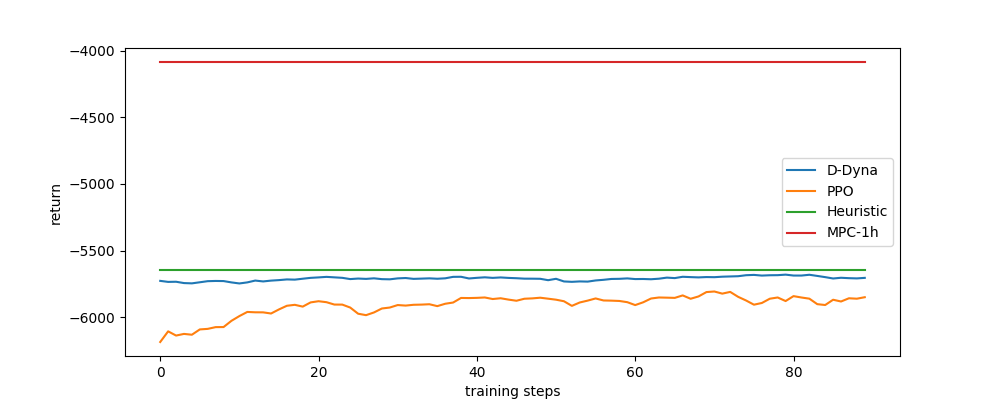
\includegraphics[width=0.8\textwidth]{aug.png}
     		\caption{Cumulative return on the August.}
			\label{fig:transfer-aug}
     	\end{minipage}
     
     \end{figure}

\section{\textbf{TODO} Conclusions} \label{sec: conclusions}
    In this paper, a novel model-based reinforcement learning algorithm is proposed for the control of a microgrid. First, an open-source reinforcement framework for the modeling of an off-grid microgrid for rural electrification is presented. The control problem of an isolated microgrid is casted as a Markov Decision Process (MDP). The proposed algorithm learns a model online using the collected experiences. This model is used to sample states during the evaluation step of the proximal policy optimization algorithm.
    
    We compare the proposed algorithm to the standard benchmarks in the literature. Firstly, a rule-based control that takes decisions in a myopic manner based only on current information and secondly an optimization-based controller with look-ahead are considered for comparison puroposes. \textcolor{red}{The proposed algorithm outperforms the myopic rule-based controller as well as the optimization based one.}
    
    Moreover, we test the generalization capabilities and the ability to transfer knowledge from one training session to the next. The results indicate that ...
    

\section{Acknowledgments}
This research is carried out in the framework of the Dynamically Evolving Long-Term Autonomy (DELTA) project.
DELTA is a European research project funded under the CHIST-ERA scheme (\url{http://www.chistera.eu/}). {\color{red} UPF has to add the specific Spanish grant as well.} The authors would like to thank Sergio Balderrama for the provision of measured data from the ''El Espino" microgrid in Bolivia and Alessandro Davide Ialongo for the fruitful discussion.


% In the unusual situation where you want a paper to appear in the
% references without citing it in the main text, use \nocite
% \nocite{langley00}

\bibliography{reference.bib}
\bibliographystyle{src/icml2020}

\section*{Appendix}

\subsection*{Notation}
\subsection*{\textit{\textbf{Set and indices}}}

\begin{itemize}
	\item $b$ battery index
	\item $g$ conventional generator index
	\item $t$ time period index
	\item $\mathcal{B}$ set of all batteries
	\item $\mathcal{G}$ set of all conventional generators
	\item $\nonsteerableDevices$ set of all non steerable generators
	\item $\nonflexibleDevices$ set of all non flexible loads
	\item $\mathcal{A}$ action space
	\item $\mathcal{S}$ state space
	\item $\OPperiods$ set of periods in the control horizon
\end{itemize}  

\vspace*{0.25cm}
\subsection*{\textit{\textbf{Parameters}}}
\begin{itemize}
	\item $\chargerate$, $\dischargerate$ maximum charge and discharge rate (kW)
	\item $\overline{\nonSteerable}$ non steerable generation (kW)
	\item $\overline{\steerable}$ steerable generator capacity (kW)
	\item $\underline{\steerable}$ minimum steerable generation (kW)
	\item $\initialCharge$ initial state of charge (kWh)
	\item $\maxcharge$, $\mincharge$ maximum and minimum battery capacity (kWh)
	\item $\OPduration$ simulation and control period duration (h)
	\item $\chargeEfficienty$, $\dischargeEfficienty$ charge and discharge efficiency (\%) 
	\item $\OPprice{curt}$ curtailment cost (\texteuro/kWh)
	\item $\OPprice{fuel}$ fuel cost (\texteuro/kWh)
	\item $\OPprice{lost load}$ lost load cost (\texteuro/kWh)

	
\end{itemize}
\subsection*{\textit{\textbf{Variables}}}
\begin{itemize}
	\item $a$ control actions vector
	\item $\charge$, $\discharge$ fraction of the maximum charging and discharging power [0,1]
	\item $\shed$, load shed
	\item $\curtail$ generation curtailed
	\item $\steer$ generation activated
	\item $\nonSteerable$ non-steerable generation
	\item $\nonFlexible$ non-flexible load
	\item $k$ binary variable 
	\item $\profit{fuel}$ fuel cost (\texteuro)
	\item $\profit{curt}$ curtailment cost (\texteuro)
	\item $\profit{shed}$ lost load cost (\texteuro)
	\item $SoC$ state of charge of battery (kWh)
	\item $\charge$ charged energy of battery (kWh)
	\item $\discharge$ discharged energy of battery (kWh)

\end{itemize}


\end{document}


% This document was modified from the file originally made available by
% Pat Langley and Andrea Danyluk for ICML-2K. This version was created
% by Iain Murray in 2018, and modified by Alexandre Bouchard in
% 2019 and 2020. Previous contributors include Dan Roy, Lise Getoor and Tobias
% Scheffer, which was slightly modified from the 2010 version by
% Thorsten Joachims & Johannes Fuernkranz, slightly modified from the
% 2009 version by Kiri Wagstaff and Sam Roweis's 2008 version, which is
% slightly modified from Prasad Tadepalli's 2007 version which is a
% lightly changed version of the previous year's version by Andrew
% Moore, which was in turn edited from those of Kristian Kersting and
% Codrina Lauth. Alex Smola contributed to the algorithmic style files.

